\begin{manpage}{\prog{plotinspiralrange}}

\manname{\prog{plotinspiralrange}}{A program for plotting inspiral horizon distance.}
\mansynopsis{\prog{plotinspiralrange}  [options] }

\begin{mansection}{Description}
\prog{plotinspiralrange} scan template bank files, 
search for horizon distance in summary table 
and create 3  pictures of horizon distance for a standard BNS first, and for
the mass range provided.  Any file whose name ends
in ``\file{.gz}'' is assumed to be gzip-compressed.

The results of the search are  stored in a png format.
\end{mansection}


\begin{mansection}{Options}
\begin{description}
\item[\progarg{--version}] show program's version number and exit
\item[\progarg{-h, --help}] show this help message and
\item[\progarg{-I INSP, --inspiral-glob=INSP}]     glob for files containing the string INSP
\item[\progarg{-c CACHE, --cache-file=CACHE}]    name of cache file with details if
\item[\progarg{-s, --show-plot}] display the figures on the
\item[\progarg{-m MIN, --range-min=MIN}]     minimum value on range plots  
\item[\progarg{-M MAX, --range-max=MAX}]     maximum value on range plots  
\item[\progarg{-a, --range-vs-time}]  make a plot of range
\item[\progarg{-b, --range-hist}]  make a histogram of the
\item[\progarg{--range-mass}]  make a plot of the range
\item[\progarg{--mass-min=MIN}]  minimum x-value on mass plots 
\item[\progarg{--mass-max=MAX}]  maximum x-value on mass plots 
\item[\progarg{-t PLOT\_TYPE, --plot-type= PLOT\_TYPE}]    make either linear or log or plots
\item[\progarg{-n NBINS, --nbins=NBINS }]    number of bins for range hist (default
\item[\progarg{-f FNAME, --figure-name= FNAME}]   generate png figures with name FNAME-fig.png 
\item[\progarg{-W, --output-html}] generate a html page containing
\item[\progarg{-C, --output-cache}] generate a cache file with
\item[\progarg{-P PATH, --output-path=PATH}]     path where the figures would be stored
\item[\progarg{-S GPSSTART, --gps-start-time=GPSSTART}]    gps start time (for naming figure and
\item[\progarg{-E GPSEND, --gps-end-time= GPSEND}]   gps end time (for naming figure and
\item[\progarg{-v, --verbose}] print information   
\end{description}
\end{mansection}


\begin{mansection}{Output}
This program returns three png images such in
figure\ref{fig:lalapps_plotinspiralrange}, an html file and a cache file (if
ouptut-html and output-cache are provided). The output filenames follow the
naming convention : 

plotinspiralrange\_usertag\_figurename-gpsstart-duration


\begin{figure}[ht]
{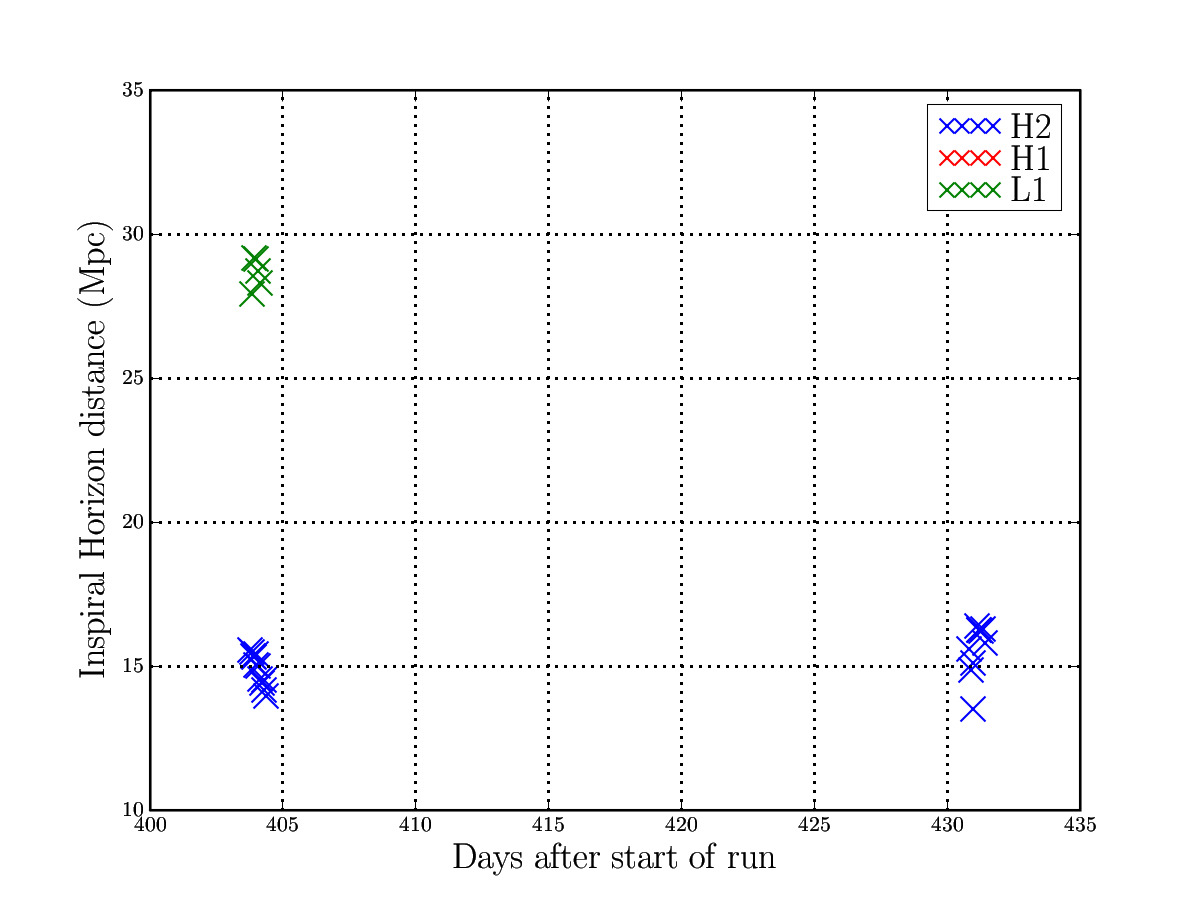
\includegraphics[width=0.30\textwidth]{./plotinspiralrange_playground_range_plot-849974770-2419200.png}}
{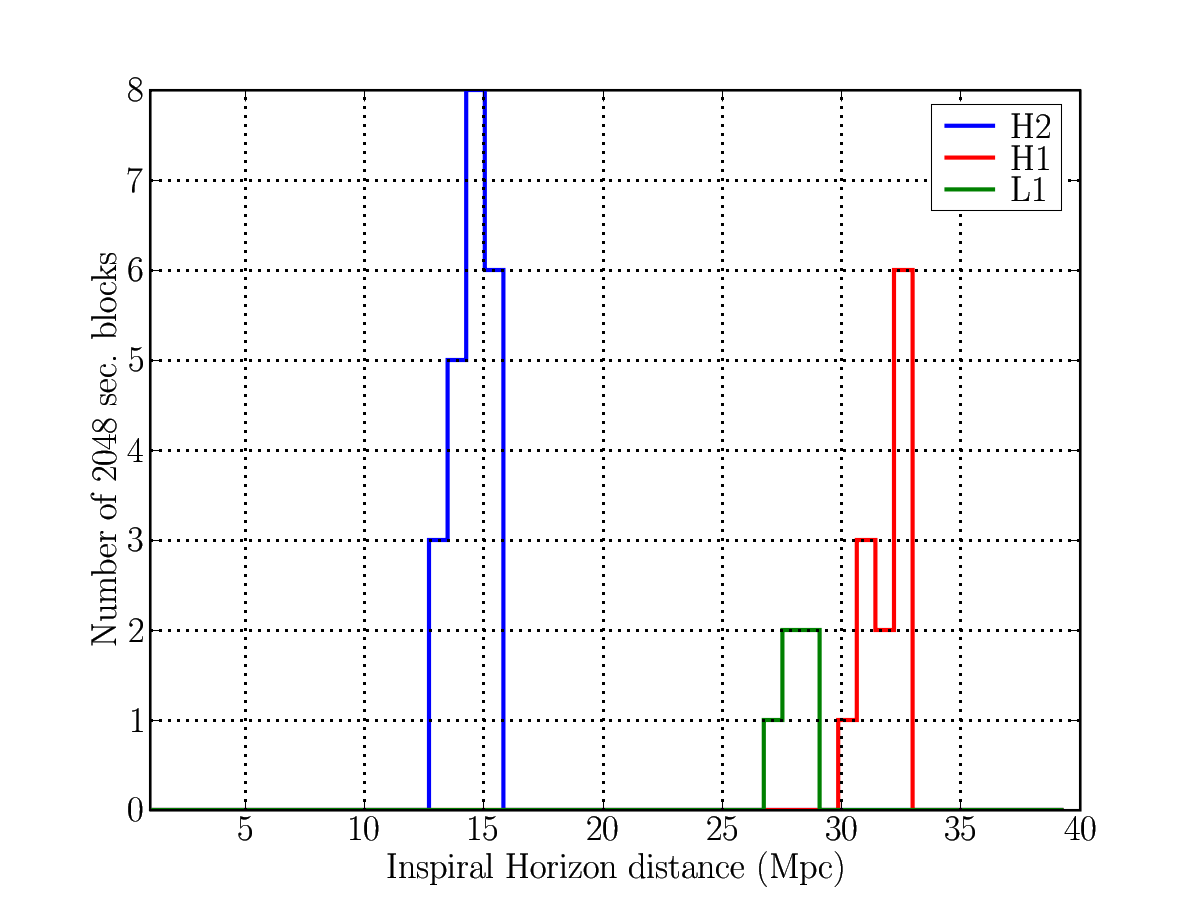
\includegraphics[width=0.30\textwidth]{./plotinspiralrange_playground_range_hist-849974770-2419200.png}}
{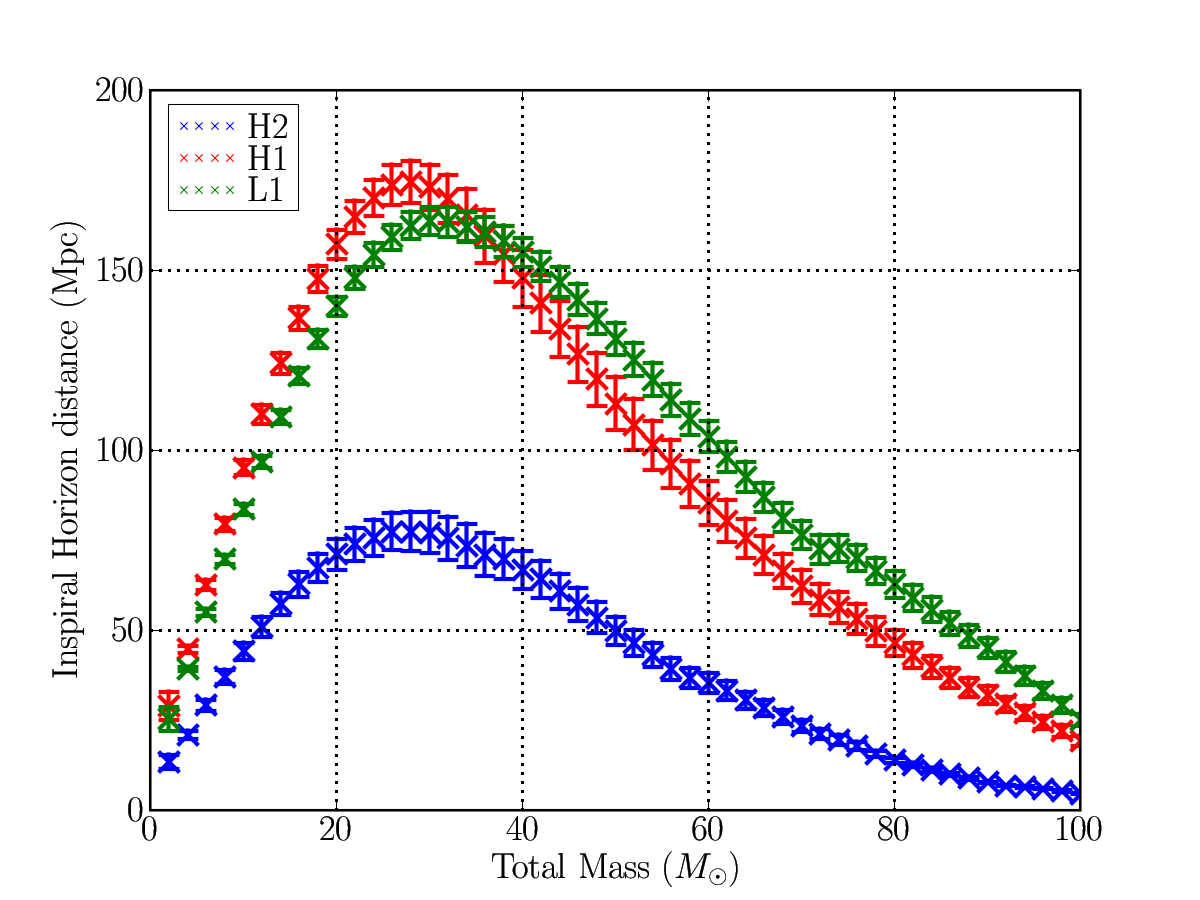
\includegraphics[width=0.30\textwidth]{./plotinspiralrange_playground_range_mass-849974770-2419200.png}}
\caption{\label{fig:lalapps_plotinspiralrange} test}
\end{figure}
\end{mansection}

\begin{mansection}{Examples}
\begin{verbatim}
~/opt/pylal/bin/lalapps_plotinspiralrange --cache-file  test.cache   -f
playground --range-min 1 --range-max 40 --n 50 --range-vs-time --range-hist
--verbose -a -b --range-mass --gps-start-time 849974770 --gps-end-time
852393970  --output-cache --output-html --output-path playground --help
\end{verbatim}
\end{mansection}



\begin{mansection}{See Also}
\prog{plotnumtriggers}, \prog{plotinspiral}
\end{mansection}

\end{manpage}

\clearpage
